\documentclass{article}
\usepackage[utf8]{inputenc}
\usepackage{graphicx}

\title{Driving Behavior}
\author{
Ernesto Adrián Álvarez Salazar  A00227490\\
Carlos Javier Leal Beltrán  A01741355\\
Carlos Moisés Chávez Jiménez  A01637322\\
Luis Armando Salazar López  A01114901\\
}
\date{Agosto 2022 - Septiembre 2022}

\usepackage{listings}
\usepackage{color}

\definecolor{dkgreen}{rgb}{0,0.6,0}
\definecolor{gray}{rgb}{0.5,0.5,0.5}
\definecolor{mauve}{rgb}{0.58,0,0.82}

\lstset{frame=tb,
  language=Python,
  aboveskip=3mm,
  belowskip=3mm,
  showstringspaces=false,
  columns=flexible,
  basicstyle={\small\ttfamily},
  numbers=none,
  numberstyle=\tiny\color{gray},
  keywordstyle=\color{blue},
  commentstyle=\color{dkgreen},
  stringstyle=\color{mauve},
  breaklines=true,
  breakatwhitespace=true,
  tabsize=3
}

\begin{document}

\maketitle

\section{Introducción}

Una conducta agresiva al manejar es el factor principal en los accidentes vehiculares en carretera. Así lo reporta la "AAA Foundation for Traffic Safety", ya que, dentro de 106,727 choques fatales en un periodo reciente de 4 años, el 55.7 \% de estos involucró a conductores que cometieron una o más acciones agresivas al manejar. Por lo anterior, buscamos ¿Cómo predecir conductas agresivas al manejar de manera rápida y lo más precisa posible?

La conducción agresiva incluye el exceso de velocidad, las pausas repentinas y los giros bruscos a la izquierda o a la derecha. Todos estos eventos se reflejan en los datos del acelerómetro y el giroscopio. Por lo tanto, sabiendo que hoy en día casi todo el mundo posee un smartphone que tiene una gran variedad de sensores, hemos obtenido diversos datos gracias a una aplicación de recopilación de datos en Android basada en los sensores del acelerómetro y el giroscopio.


\section{Tratamiento Inicial de los Datos}

Para comenzar a trabajar con los datos, es necesario que pasen por un proceso de preparación que nos permita obtener la mejor parte de ellos. Este proceso se divide en tres etapas: Limpieza, Transformación y Visualización. A continuación desglosaremos las fases involucradas a este proceso:

    \subsection{Limpieza de los datos}

        La limpieza es la primera y una etapa fundamental del tratamiento de la información. Aquí se busca eliminar la mayor cantidad de imperfecciones que pudiéramos llegar a encontrar. Cosas como valores faltantes, datos fuera de rango, dividir la información disponible en "entrenamiento" y "pruebas", eliminar columnas innecesarias para el análisis, etc.
        
        En el caso de nuestra base de datos, no hicimos ninguna limpieza (de momento). Encontramos muchos valores atípicos en las variables relacionadas con el movimiento de los conductores (giroscopio y acelerómetro), pero no los eliminamos. Al ser demasiados, puede generar que se vaya mucha información que resulte valiosa para nuestro modelo. La parte importante fue que no encontramos valores faltantes, ni columnas innecesarias. \\

        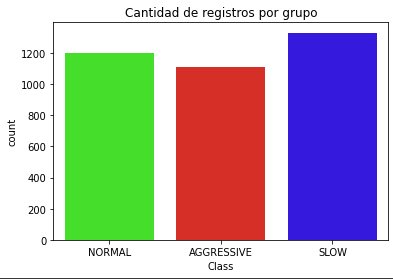
\includegraphics{images/Columnas.png} \\

        \textbf{Gráfico de barras sobre las clases disponibles en nuestro archivo de datos.} \\

    \subsection{Transformación de los datos}

        Una vez revisados los datos, entendemos que debemos transformarlos para generar gráficos y diagramas que faciliten la búsqueda de patrones y la determinación de si será necesario un modelo predictor de regresión o de clasificación.
        
        Para esto, revisamos el dataframe con la información proporcionada. Encontramos que primero debemos ordenar los datos con base en el timestamp. Esta variable indica el tiempo con el que fueron realizadas las pruebas de los conductores. Se generaron dos observaciones por segundo, lo que indica que tenemos que separarlas para que queden enumeradas de uno en uno. Le restamos el primer valor del timestamp a todas las observaciones para dejar la inicial en 0, y separamos los valores para que quedaran enumeradas por el número de observación y no por el tiempo. Así no habría dos observaciones en el mismo segundo.
        
        En cuanto a lo demás, los datos venían en buenas condiciones, por lo que no tuvimos que arreglar valores nulos, ni valores que vinieran en formatos con los que no se puede trabajar.

    \subsection{Visualización de los datos}

       Esta etapa es un caso diferente. Pertenece igualmente a las fases previas al trabajo de los datos, pero no involucra descartar información. La visualización se encarga convertir los datos a diagramas o elementos gráficos que faciliten el entendimiento de la información. También para esta fase consideramos el cambiar algunas variables de tipo de dato.

        Con base en los datos que contamos para realizar este trabajo, analizamos y decidimos qué diagramas utilizar para acercarnos al desarrollo de nuestro modelo. Seleccionamos los diagramas de correlación y cajas y bigotes. \\
        El diagrama de correlación nos permite conocer qué variables son más afines a la variable que estamos intentado predecir. Lo cual nos ahorra mucho trabajo para seleccionar las variables que estarán involucradas en nuestro modelo. \\

        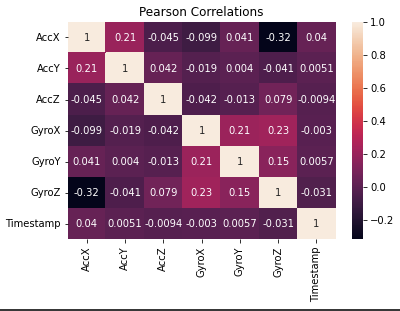
\includegraphics{images/Correlacion.png} \\

        \textbf{Gráfico de correlación entre nuestras variables.} \\
        
        El diagrama de cajas y bigotes nos permitió conocer si hay valores atípicos en nuestros datos con respecto a las variables independientes. De esta forma nosotros podemos descartar estos valores para hacer un modelo más ajustado y apegado a la realidad. Pero, para este caso particular, no debemos hacerlo. Al ser tantos este tipo de valores, el eliminarlos podría maquillar los datos y generar un modelo erróneo.\\

        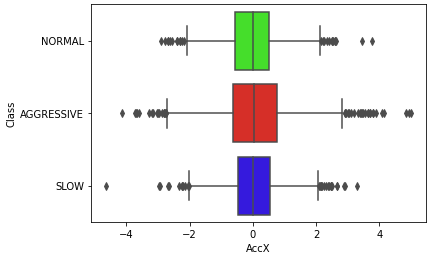
\includegraphics{images/Cajas y Bigotes AccX.png} \\

        \textbf{Gráfico de cajas y bigotes sobre la variable de aceleración "Acc X".} \\

\section{Desarrollo del modelo con los datos}

Habiendo trabajado ya con las primeras partes de los datos, ya podemos sacar conclusiones en cuanto a los patrones que buscamos, el cómo vamos a trabajar con los datos, cuántos datos requerimos para predecir y qué modelo elegir. \\
        
    \subsection{Busqueda de patrones}

        La visualización nos permitió entender que no estamos buscando un modelo nos prediga una clase con base a los parámetros, sino un conjunto de observaciones que nos permita clasificar el tipo de conductor con base en la información de como conduce. 
        
        Al momento de analizar los gráficos que obtuvimos de los datos, encontramos algunos comportamientos y patrones que nos pueden acercar al desarrollo del modelo. Vimos que el comportamiento del conductor agresivo es cambiante constantemente y extremo en cuanto a los cambios de aceleración y dirección en todas las dimensiones. Para comprobar esto, sacamos el valor total de las tres dimensiones de la aceleración y el giro para generar un gráfico que nos permita verificar que sí hay cambios observables entre los conductores.

        \includegraphics{images/Aceleración Total.png} \\

        \textbf{Gráfico de Lineas sobre la suma de las aceleraciones en las tres dimensiones del acelerómetro.} \\

        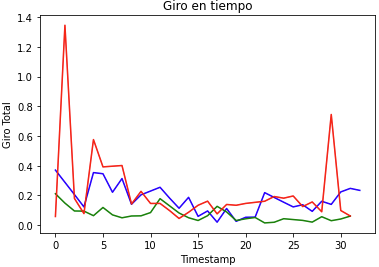
\includegraphics{images/Giro Total.png} \\

        \textbf{Gráfico de Lineas sobre la suma del giro en las tres dimensiones del giroscopio.} \\

        Como vimos en los anteriores gráficos, notamos que los valores del conductor agresivo se disparan y cambian constantemente. Esto simplemente nos muestra que nuestra idea inicial en cuanto a la inestabilidad y capacidad de predicción con base en los cambios de aceleración y el giro se comprueba. Lo anterior nos da una idea de lo que buscamos en nuestro modelo, y nos da una pauta de lo que podemos hacer para generar un modelo eficiente.

        Otra cosa que también nos ayudó a encontrar patrones, fue el sacar la raíz de las sumatorias de los cuadrados y las aceleraciones. De esta forma obtenemos un valor único para la aceleración y el giro de cada dirección. Los resultados que obtuvimos fueron los siguientes: \\

        \begin{center}
        \begin{tabular}{||c c c c||} 
         \hline
         Clase & X & Y & Z \\ [0.5ex] 
         \hline\hline
         Agresivo - Acc & 31.38 & 26.88 & 31.62 \\ 
         \hline
         Medio - Acc & 30.00 & 28.22 & 33.42 \\
         \hline
         Lento - Acc & 40.75 & 38.39 & 37.66 \\
         \hline
         Agresivo - Giro & 2.49 & 4.57 & 3.76 \\
         \hline
         Medio - Giro & 2.10 & 4.07 & 3.95 \\ [1ex] 
         \hline
         Lento - Giro & 2.39 & 4.53 & 4.39 \\ [1ex] 
         \hline
        \end{tabular}
        \end{center}

        Analizando los resultados, el giro no nos dijo mucho en cuanto a diferencias. Los datos son muy parecidos en cuanto a los tres tipos de conductores. Pero, podemos ver que sí hay una diferencia notable en la aceleración. Específicamente en las dimensiones Y y Z. Lo cual nos indica que podemos utilizar esas variables representativas para probar diferentes modelos y obtener el que tenga una mayor eficiencia.
        

    \subsection{Metodología}

        Para comenzar el desarrollo fue necesario primero definir si el modelo fuese de regresión o de clasificación. Determinamos que debe ser de clasificación porque nosotros esperamos recibir determinada cantidad de observaciones tomadas del manejo de un conductor, y determinar qué tipo de conductor es. Teniendo definido lo anterior, es importante establecer cuántas observaciones serán necesarias para que el modelo haga la predicción. 
        
        Para calcular la cantidad de observaciones suficientes pensamos en que lo mejor es definirlo con base en los datos que nos dan para test. Dividiendo la cantidad de datos entre las tres clases, ajustamos los datos para que nos den valores divisores similares. De esta forma encontramos el máximo común divisor de los datos y así determinamos la cantidad mínima de datos que necesitamos de un conductor para determinar si puede llegar a ser peligroso para los otros automovilistas.

        Teniendo los datos listos para trabajar, establecida la cantidad de datos mínima, con los patrones descubiertos y la idea de lo que buscamos definida; comenzaremos la búsqueda del modelo con la mayor eficiencia. Dentro de los modelos que probaremos están \textbf{Random Forest} , \textbf{KNN} y \textbf{Decision Tree}.

        \subsubsection{Decision Tree}

            El primer candidato es el árbol de decisión. Este divide los datos entre todas sus características para clasificar al valor que se ingresa en una categoría. 
            
            Siendo el caso de nuestros conductores, el modelo crea diferentes nodos de decisión donde se va clasificando el dato hasta que encaje con las características de un conductor. 

            Algunas ventajas de este candidato son que es muy fácil de entender el funcionamiento, es válido tanto para variables cuantitativas y cualitativas y no requiere amplia preparación de los datos.

            Una de sus desventajas es que es inestable, un cambio en los datos desencadenaría en una reorganización del árbol.

            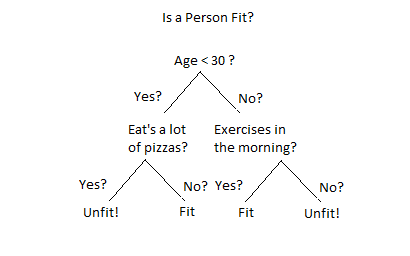
\includegraphics[scale=0.8]{images/decisionTree.png} \\

            \textbf{Ejemplo de decision tree.}
            

        \subsubsection{KNN}

            Es un algoritmo clasificador de aprendizaje supervisado no paramétrico. Este utiliza la proximidad para hacer clasificaciones o predicciones sobre la agrupación de un punto de datos individual. Aunque se puede utilizar para problemas de regresión o clasificación, por lo general se utiliza como un algoritmo de clasificación, iniciando de la suposición en la que se pueden encontrar puntos similares cerca uno del otro. Cada vez que se agrega una nueva observación se utiliza la etiqueta que se representa con más frecuencia alrededor de este punto de datos determinado.

            Algunas de sus ventajas son que es un algoritmo simple de entender y que, al no ser paramétrico, no realiza suposiciones específicas sobre la forma funcional de los datos, evitando así los peligros de una distribución subyacente de los datos.

            Pero, sus principales desventajas es que es un algoritmo muy costoso de almacenamiento, porque tiene que guardar todos los datos de entrenamiento, y que está basado en instancia. Esto significa que el algoritmo no aprende explícitamente un modelo, en su lugar, prefiere memorizar las instancias de capacitación que se utilizan después como conocimiento para la fase de predicción.

            \begin{figure}[ht]
            \centering
                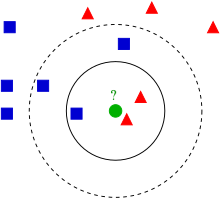
\includegraphics[scale=0.9]{images/knnEx.png} \\
                \textbf{Ejemplo de KNN.} \\
            \end{figure}

        \subsubsection{Random Forest}

            Por último, está Random Forest. Este desarrolla múltiples árboles de decisión y los combina para obtener una predicción más precisa y estable. En general, mientras más árboles haya en el bosque, más robusto será.

            En este algoritmo se agrega algo aleatoriedad adicional al modelo, mientras crece los árboles, en lugar de solo buscar la característica más importante al dividir un nodo, busca la mejor característica entre un subconjunto aleatorio de características. Lo cual nos da como resultado una amplia diversidad que por lo general resulta en un mejor modelo.
    
            Una de sus ventajas es que funciona muy bien aún sin pasarle hiperparametros. Otra cosa es que es muy estable con su funcionamiento, no se desestabiliza cuando modificas los datos. Es ideal para dataset grandes, ya que entre más arboles contenga, menos overfiting tendrá.
    
            Su desventaja principal es que puede llegar a ser muy costoso comparado con un simple árbol de decisión. Por la misma razón, no funciona correctamente con datasets pequeños. \\

            \begin{figure}[ht]
            \centering
                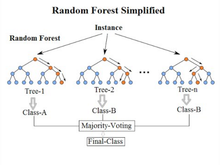
\includegraphics[scale=1.6]{images/RandomF.png} \\
                \textbf{Ejemplo de Random Forest.} \\
            \end{figure}

\section{Resultados}

Habiendo entendido las metodologías de los tres tipos de modelo que utilizamos, vamos a poner a prueba su efectividad y compararemos sus resultados:

    \begin{center}
    \begin{tabular}{||c c||} 
     \hline
     Modelo & Efectividad \\ [0.5ex] 
     \hline\hline
     Knn - AccY y AccZ Var & 57.38 \\ 
     \hline
     Decision Tree - Todas Var & 49.18 \\
     \hline
     Random Forest - AccY Var & 60.66 \\
     \hline
     Random Forest - Todas Var & 68.85 \\
     \hline
    \end{tabular}
    \end{center}

Como podemos ver tenemos una mayor efectividad en los modelos de random forest. Lo cual puede ser un gran indicio para indicar que nos debemos decantar por el modelo con mayor efectividad. Pero, no es del todo así.


En este análisis estamos buscando identificar a los conductores agresivos con base en sus datos, para que tomen sus precauciones con respecto a su forma de manejar. Por esta razón no podemos quedarnos simplemente con un modelo efectivo para clasificar a un conductor, debemos encontrar el mejor para identificar agresivos. Para esto vamos a generar una matriz de confusión que nos permitirá ver cuántas veces es capaz de clasificar correctamente conductores agresivos para cada modelo, y de esa manera seleccionar el mejor modelo para nosotros. Los resultados son los siguientes:

    \subsubsection{Decision Tree - Todas las variables}

        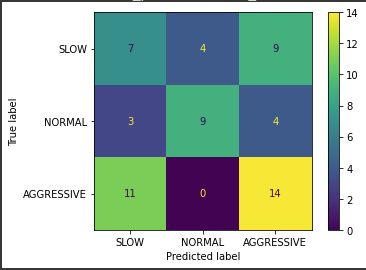
\includegraphics{images/MatrizDecision.png} \\

        \textbf{Matriz de confusión del modelo Arboles de Decisión.} \\

    \subsubsection{KNN - Solo variables ACCY y ACCZ}

        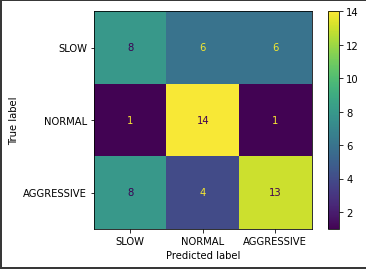
\includegraphics{images/MatrizKnn.png} \\

        \textbf{Matriz de confusión del modelo KNN utilizando solo las dos variables con mejor correlación.} \\

    \subsubsection{Random Forest - Solo variable ACCY}

        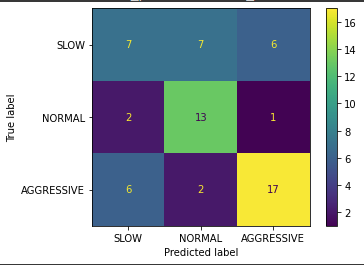
\includegraphics{images/MatrizAgg.png} \\

        \textbf{Matriz de confusión del modelo Random Forest solo usando la variable con la mejor correlación.} \\

    \subsubsection{Random Forest - Todas las variables}

        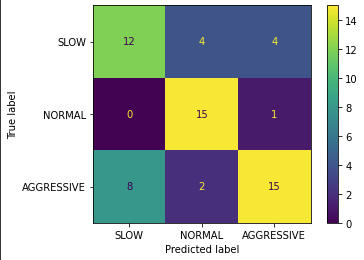
\includegraphics{images/MatrizMejor.png} \\

        \textbf{Matriz de confusión del modelo Random Forest solo usando todas las variables.} \\

Estas matrices de confusión son muy claras en cuando a los resultados. Podemos notar que el modelo más efectivo (Random Forest con todas las variables) no es el que mejor predice a los conductores agresivos. En cambio, el que no es tan efectivo (Random Forest univariable con ACCY), predice mejor a los conductores agresivos.

    \subsection{Conclusiones Finales}
            
            Al final, pudimos detectar el mejor modelo para nuestro objetivo. Este tiene una efectividad del 60.66 \% identificando tipos de conductores, pero del 68 \% identificando conductores agresivos. La razón por la que el modelo no tiene una efectividad del 100 \% es porque tiene muchos valores fuera de rango. La inconsistencia en los datos tiene un impacto grande al momento de entrenar e intentar predecir. Al ser muy alta la cantidad de valores de este tipo, la generación de un análisis eficiente se hace más complicada. Dejando de lado esto, el modelo es lo suficientemente preciso para poder identificar a gran parte de estos conductores y evitar una gran cantidad de accidentes. 

            Creemos que esta es una forma eficaz para disminuir los accidentes automovilísticos y el atropellamiento de peatones. Prevenir a la población de conductas agresivas durante el tráfico es primordial para no ser parte del problema y comenzar a adoptar técnicas de control de emociones y de prevención de accidentes.

\end{document}
